% Adjust these for the path of the theme and its graphics, relative to this file
%\usepackage{beamerthemeFalmouthGamesAcademy}
\usepackage{../../beamerthemeFalmouthGamesAcademy}
\usepackage{multimedia}
\graphicspath{ {../../} }

% Default language for code listings
\lstset{language=C++,
        morekeywords={each,in,nullptr}
}

% For strikethrough effect
\usepackage[normalem]{ulem}
\usepackage{wasysym}

\usepackage{pdfpages}

% http://www.texample.net/tikz/examples/state-machine/
\usetikzlibrary{arrows,automata}

\newcommand{\modulecode}{COMP260}\newcommand{\moduletitle}{Distributed Systems}\newcommand{\sessionnumber}{5}

\begin{document}
\title{\sessionnumber: Presence}
\subtitle{\modulecode: \moduletitle}

\frame{\titlepage} 

\begin{frame}
	``We see things not as they are, but as we are - that is, we see the world not as it is, but as moulded by the individual peculiarities of our mind'' - Philosopher, G.T.W Patrick. (1890) \\~\\
	\pause
	Reality is malleable. \\~\\ 
	\pause
	Our point of view is inseparable from our understanding of reality. 	
	
\end{frame}


\begin{frame}
	\frametitle{Presence (again)}
	
	`Presence is the psychological state of subjective perception in which even though part or all of an individual's current experience is generated by and/or filtered through human-made technology, part or all of the individual's perception fails to accurately acknowledge the role of the technology in the experience.' \\~\\
	
	International Society for Presence Research, 2000
	\\~\\
	\href{http://ispr.info}{[ISPR Website]}	
	
\end{frame}

\begin{frame}
	\begin{center}
		\href{https://www.youtube.com/watch?v=gvozcv8pS3c}{ 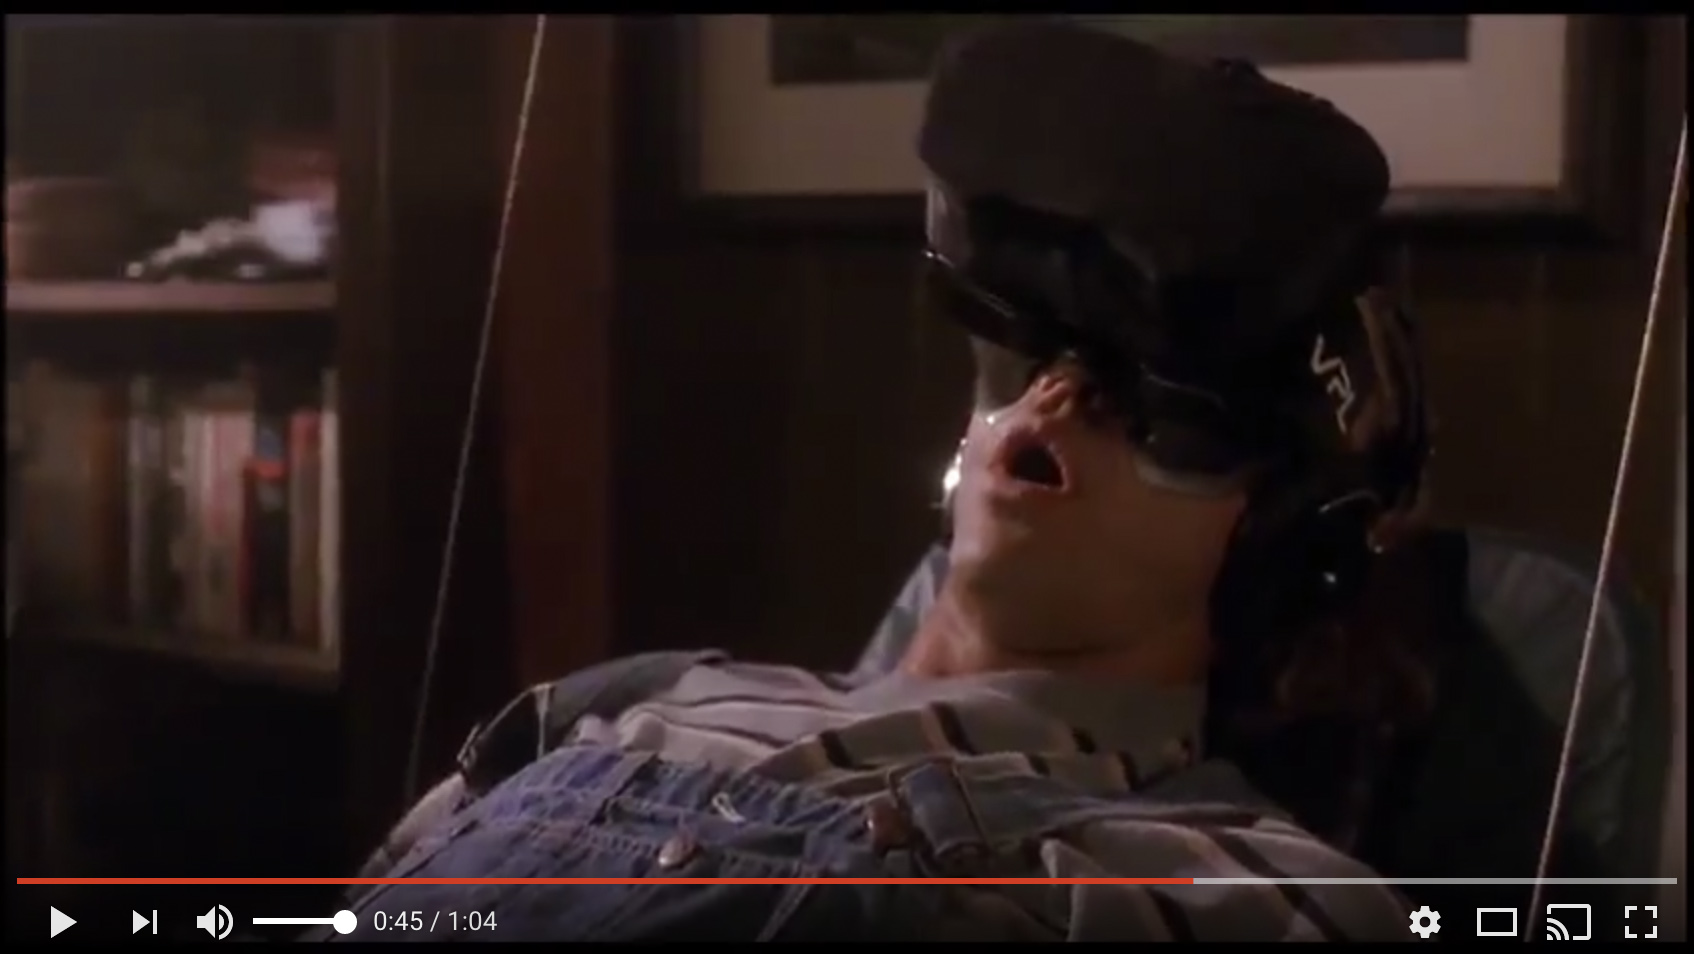
\includegraphics[scale=.3]{assets/mower}  }
	\end{center}
\end{frame}

\begin{frame}
	\frametitle{Duck Test}
	
\end{frame}
	

\begin{frame}
	\frametitle{Illusions}
	V/AR are illusion based experiences \\~\\ 
	
	There are four main components to this illusion:
	\begin{itemize}
		\item the stable spacial place,
		\item self-embodiment,
		\item physical interaction \&,
		\item social communication.
	\end{itemize}
	
\end{frame}

\begin{frame}
	\frametitle{The Uncanny Valley}
	\begin{figure}
		 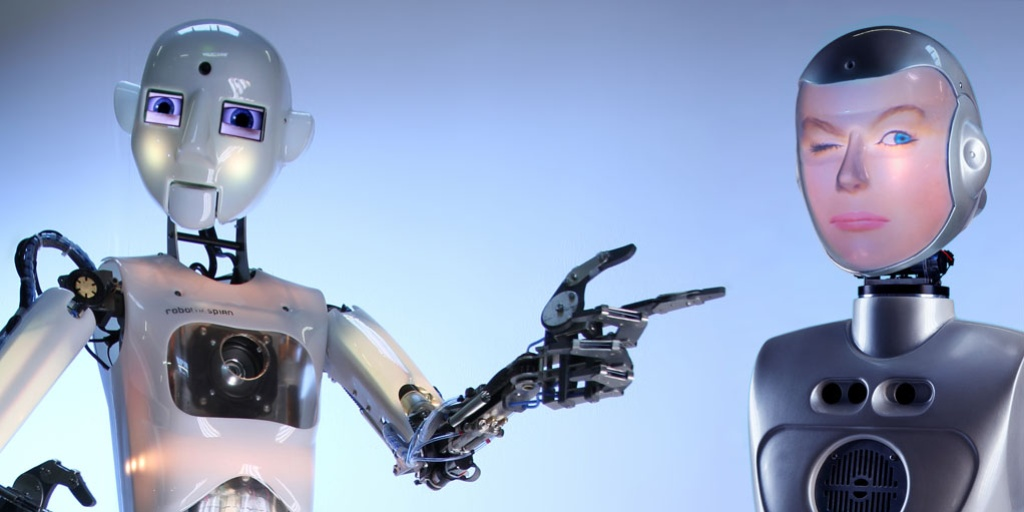
\includegraphics[scale=.3]{assets/bots}  
		 \caption{Engineered Arts - Penryn}
	\end{figure}
\end{frame}

\begin{frame}
	\begin{figure}
		 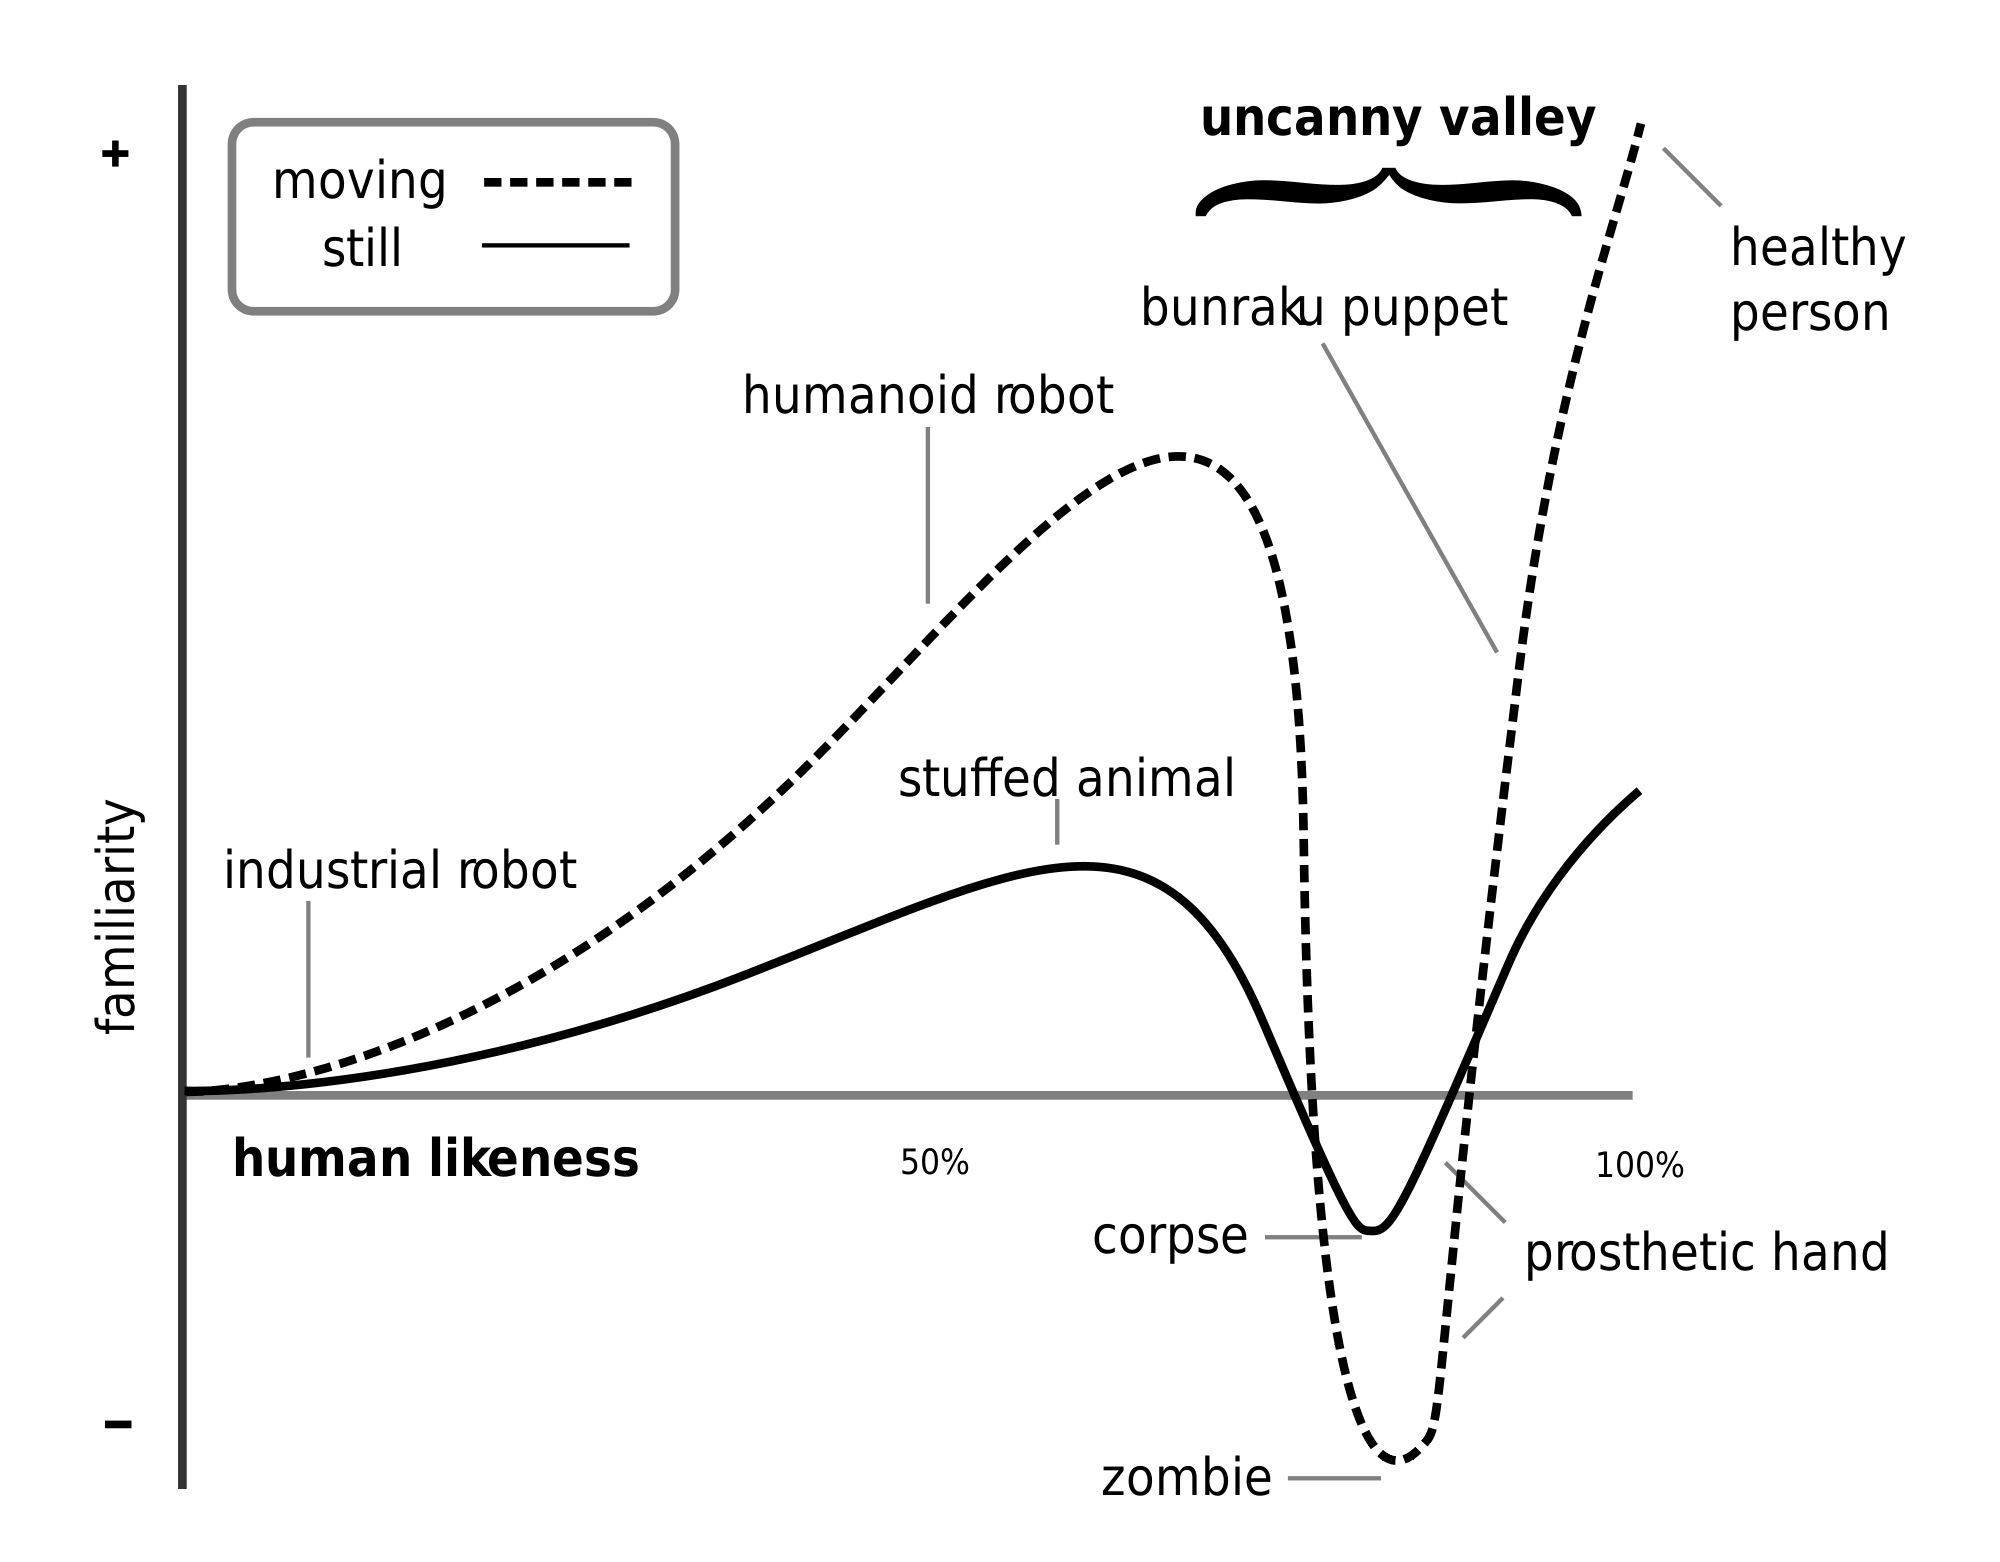
\includegraphics[scale=.13]{assets/uncanny}  
		  \caption{Masahiro Mori - }
	\end{figure}
\end{frame}

\begin{frame}
	\frametitle{Fidelity Continua}
	The notion of the uncanny valley applies to aspects of VR as well. These components have been defined as the Fidelity Continua. 
	
	\begin{itemize}
	 	\item	\textbf{Representation} fidelity - Hyper-realistic to abstract and non-objective worlds. 
		\item	\textbf{Interaction} Fidelity - Degree to which a interaction in VR corresponds with the same interaction in the real world.
		\item \textbf{Experiential} Fidelity - The degree to which the user experience matches the intentions of the VR creator. Procedural worlds have a very low experiential fidelity.
	 \end{itemize}
		
\end{frame}

\begin{frame}
	What do we want from V/AR? \\~\\
	Some aim to recreate reality to the highest fidelity. \\~\\
	Others seek to surpass it.
\end{frame}


\begin{frame}
	\frametitle{Perception}
\end{frame}

\begin{frame}
	\frametitle{Objective vs. Subjective Reality}
	
\end{frame}


\begin{frame}
	\begin{figure}
		\href{https://www.youtube.com/watch?v=qD3w3cAhEYU}{ 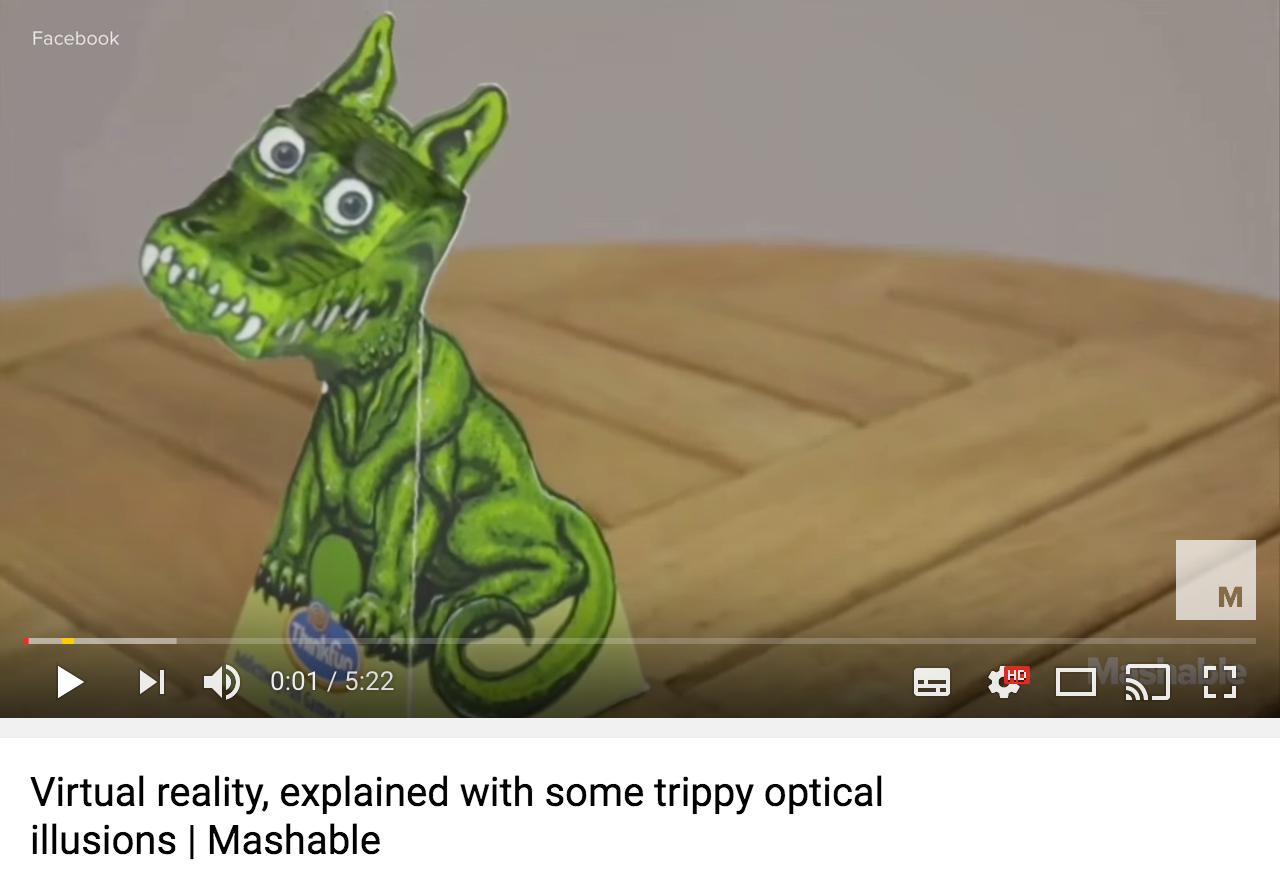
\includegraphics[scale=.4]{assets/optical}  }
		\caption{Michael Abrash, the chief scientist for Facebook's Oculus}
	\end{figure}
\end{frame}

\begin{frame}
	\frametitle{Human-Centred Design}
	
\end{frame}

\begin{frame}
	\frametitle{Learning outcomes}
	\begin{itemize}
		\item Outcome 1
		\item Outcome 2
		\item Outcome 3
	\end{itemize}
\end{frame}

\begin{frame}
	\frametitle{Sensory Substitution}
	Sensory substitution is the replacement one sensory cue that is not yet able to be simulated with one that is. The majority of the time the replacement relies on the dominance of sight. (sight is more dominant than proprioception and so on)

\end{frame}


\begin{frame}
	\frametitle{Redirected Walking}
\end{frame}

\end{document}
